% -*- coding: utf-8 -*-
%-------------------------designed by zcf--------------
\documentclass[UTF8,a4paper,10pt]{ctexart}
\usepackage[left=3.17cm, right=3.17cm, top=2.74cm, bottom=2.74cm]{geometry}
\usepackage{amsmath}
\usepackage{graphicx,subfig}
\usepackage{float}
\usepackage{cite}
\usepackage{caption}
\usepackage{enumerate}
\usepackage{booktabs} %表格
\usepackage{multirow}
\usepackage{minted}
\usemintedstyle{xcode}
\usepackage{svg}
\newcommand{\tabincell}[2]{\begin{tabular}{@{}#1@{}}#2\end{tabular}}  %表格强制换行
%-------------------------字体设置--------------
% \usepackage{times} 
\usepackage{ctex}
\setCJKmainfont[ItalicFont=Noto Sans CJK SC Bold, BoldFont=Noto Serif CJK SC Black]{Noto Serif CJK SC}
\newcommand{\yihao}{\fontsize{26pt}{36pt}\selectfont}           % 一号, 1.4 倍行距
\newcommand{\erhao}{\fontsize{22pt}{28pt}\selectfont}          % 二号, 1.25倍行距
\newcommand{\xiaoer}{\fontsize{18pt}{18pt}\selectfont}          % 小二, 单倍行距
\newcommand{\sanhao}{\fontsize{16pt}{24pt}\selectfont}  %三号字
\newcommand{\xiaosan}{\fontsize{15pt}{22pt}\selectfont}        % 小三, 1.5倍行距
\newcommand{\sihao}{\fontsize{14pt}{21pt}\selectfont}            % 四号, 1.5 倍行距
\newcommand{\banxiaosi}{\fontsize{13pt}{19.5pt}\selectfont}    % 半小四, 1.5倍行距
\newcommand{\xiaosi}{\fontsize{12pt}{18pt}\selectfont}            % 小四, 1.5倍行距
\newcommand{\dawuhao}{\fontsize{11pt}{11pt}\selectfont}       % 大五号, 单倍行距
\newcommand{\wuhao}{\fontsize{10.5pt}{15.75pt}\selectfont}    % 五号, 单倍行距
%-------------------------章节名----------------
\usepackage{ctexcap} 
\CTEXsetup[name={,、},number={ \chinese{section}}]{section}
\CTEXsetup[name={(,)},number={\chinese{subsection}}]{subsection}
\CTEXsetup[name={,.},number={\arabic{subsubsection}}]{subsubsection}
%-------------------------页眉页脚--------------
\usepackage{fancyhdr}
\pagestyle{fancy}
\lhead{\kaishu \leftmark}
% \chead{}
\rhead{\kaishu 编译系统原理报告}%加粗\bfseries 
\lfoot{}
\cfoot{\thepage}
\rfoot{}
\renewcommand{\headrulewidth}{0.1pt}  
\renewcommand{\footrulewidth}{0pt}%去掉横线
\newcommand{\HRule}{\rule{\linewidth}{0.5mm}}%标题横线
\newcommand{\HRulegrossa}{\rule{\linewidth}{1.2mm}}
%-----------------------伪代码------------------
\usepackage{algorithm}  
\usepackage{algorithmicx}  
\usepackage{algpseudocode}  
\floatname{algorithm}{Algorithm}  
\renewcommand{\algorithmicrequire}{\textbf{Input:}}  
\renewcommand{\algorithmicensure}{\textbf{Output:}} 
\usepackage{lipsum}  
\makeatletter
\newenvironment{breakablealgorithm}
  {% \begin{breakablealgorithm}
  \begin{center}
     \refstepcounter{algorithm}% New algorithm
     \hrule height.8pt depth0pt \kern2pt% \@fs@pre for \@fs@ruled
     \renewcommand{\caption}[2][\relax]{% Make a new \caption
      {\raggedright\textbf{\ALG@name~\thealgorithm} ##2\par}%
      \ifx\relax##1\relax % #1 is \relax
         \addcontentsline{loa}{algorithm}{\protect\numberline{\thealgorithm}##2}%
      \else % #1 is not \relax
         \addcontentsline{loa}{algorithm}{\protect\numberline{\thealgorithm}##1}%
      \fi
      \kern2pt\hrule\kern2pt
     }
  }{% \end{breakablealgorithm}
     \kern2pt\hrule\relax% \@fs@post for \@fs@ruled
  \end{center}
  }
\makeatother
%------------------------代码-------------------
\usepackage{xcolor} 
\usepackage{listings} 
\lstset{ 
breaklines,%自动换行
basicstyle=\small,
escapeinside=``,
keywordstyle=\color{ blue!70} \bfseries,
commentstyle=\color{red!50!green!50!blue!50},% 
stringstyle=\ttfamily,% 
extendedchars=false,% 
linewidth=\textwidth,% 
numbers=left,% 
numberstyle=\tiny \color{blue!50},% 
frame=trbl% 
rulesepcolor= \color{ red!20!green!20!blue!20} 
}
%------------超链接----------
\usepackage[colorlinks,linkcolor=black,anchorcolor=blue]{hyperref}
%------------------------TODO-------------------
\usepackage{enumitem,amssymb}
\newlist{todolist}{itemize}{2}
\setlist[todolist]{label=$\square$}
% for check symbol 
\usepackage{pifont}
\newcommand{\cmark}{\ding{51}}%
\newcommand{\xmark}{\ding{55}}%
\newcommand{\done}{\rlap{$\square$}{\raisebox{2pt}{\large\hspace{1pt}\cmark}}\hspace{-2.5pt}}
\newcommand{\wontfix}{\rlap{$\square$}{\large\hspace{1pt}\xmark}}
%------------------------水印-------------------
\usepackage{tikz}
\usepackage{xcolor}
\usepackage{eso-pic}

\newcommand{\watermark}[3]{\AddToShipoutPictureBG{
\parbox[b][\paperheight]{\paperwidth}{
\vfill%
\centering%
\tikz[remember picture, overlay]%
  \node [rotate = #1, scale = #2] at (current page.center)%
    {\textcolor{gray!80!cyan!30!magenta!30}{#3}};
\vfill}}}

%———————————————————————————————————————————正文———————————————————————————————————————————————
%----------------------------------------------
\begin{document}
\begin{titlepage}
  \begin{center}
    
\includegraphics[width=0.8\textwidth]{figure/NKU.png}\\[1cm]
    \textsc{\Huge \kaishu{\textbf{南\ \ \ \ \ \ 开\ \ \ \ \ \ 大\ \ \ \ \ \ 学}} }\\[0.9cm]
    \textsc{\huge \kaishu{\textbf{计\ \ 算\ \ 机\ \ 学\ \ 院}}}\\[0.5cm]
    \textsc{\Large \textbf{预备工作2}}\\[0.8cm]
    \HRule \\[0.9cm]
    { \LARGE \bfseries 定义编译器 \& 汇编编程}\\[0.4cm]
    \HRule \\[2.0cm]
    \centering
    \textsc{\LARGE 丁屹、卢麒萱\kaishu{\ \ \ \ }}\\[0.5cm]
    \textsc{\LARGE \kaishu{年级\ :\ 2020级}}\\[0.5cm]
    \textsc{\LARGE \kaishu{专业\ :\ 计算机科学与技术}}\\[0.5cm]
    % \textsc{\LARGE \kaishu{指导教师\ :\ XX}}\\[0.5cm]
    \vfill
    {\Large \today}
  \end{center}
\end{titlepage}
%-------------摘------要--------------
\newpage
\thispagestyle{empty}
\renewcommand{\abstractname}{\kaishu \sihao \textbf{摘要}}
\begin{abstract}

  \noindent  %顶格
  \textbf{\\\ 关键字:CFG设计\ ARM汇编}\textbf{} \\\ \\\
\end{abstract}
%----------------------------------------------------------------
\tableofcontents
%----------------------------------------------------------------
\newpage
\watermark{60}{10}{NKU}
\setcounter{page}{1}

\section{总体设计及分工}
经过讨论,确定我们实现的编译器 SysY 语言特性有:
\begin{enumerate}
  \item 变量/常量声明:支持 int、float类型
  \item 数组声明:支持 int、float类型及数组指针
  \item 赋值语句
  \item 复合语句
  \item if 分支语句
  \item for/while 循环语句
  \item 算术表达式:支持加减乘除、按位与或
  \item 关系运算表达式:支持不等、等于、大于、小于
  \item 逻辑表达式:支持逻辑与或
  \item 函数
\end{enumerate}

其中,卢麒萱负责 4、5、6、7、8、9、10 的 CFG 设计,并编写了一个涵盖部分特性的简单 ARM 汇编程序;丁屹负责 1、2、3 的 CFG设计,并编写了一个涵盖了所有特性的复杂 ARM 汇编程序。

\section{CFG 描述}
\subsection{标识符及数字}
\begin{gather*}
  id \rightarrow id-nondigit\ |\ \it{id}\ id-nondigit\  |\ \it{id}\ number\\
  id-nondigit \rightarrow \rm\bf{\{\_A-Za-z\}}\\
  digit \rightarrow number\ digit\\
  number \rightarrow\ \rm\bf{\{0-9\}}\\
\end{gather*}

id 表示标识符,以下都认为为终结符,num 表示数字字符,digit 表示数字。
同名标识符的约定:
\begin{itemize}
  \item 全局变量和局部变量的作用域可以重叠,重叠部分局部变量优先;同名局
        部变量的作用域不能重叠;
  \item 变量名可以与函数名相同。
\end{itemize}

\subsection{变量/常量声明}
\begin{gather*}
  type \rightarrow \rm\bf{int\ |\ float}\\
  idlist \rightarrow idlist, \rm\bf{id\ |\ id}\\
  decl \rightarrow type\ idlist
\end{gather*}

其中 type 代表变量类型,decl 代表声明语句,idlist 代表标识符列表。

\subsection{数组声明}
\begin{gather*}
  arr\_decl\rightarrow type\ arr\_idlist\\
  arr\_idlist\rightarrow arr\_idlist,\rm\bf{id}\it{[arr\_size]}\ |\ \rm\bf{id}\it{[arr\_size]}\ |\ *\rm\bf{id} \\
  arr\_size\rightarrow \rm\bf{id}\ |\ number\ |\ \epsilon
\end{gather*}
其中 arr\_decl 代表数组声明语句,arr\_idlist 表示数组标识符列表,arr\_size 表示数组定义大小。

\subsection{赋值语句}
\begin{gather*}
  unary\_expr \rightarrow digit\ |\ \rm\bf{id}\\
  assign\_expr \rightarrow unary\_expr=assign\_expr\ |\ logical\_expr\\
  unary\_expr\rightarrow prim\_expr\ |\ funcname(paralist)\ |\ unary\_op\ unary\_expr\\
  prim\_expr\rightarrow (add\_expr)\ |\ Lval\ |\ number\\
  L\_val\rightarrow \rm\bf{id}\ \it{[exp]}\\
  unary\_op \rightarrow \rm\bf{\{+,-,!\}}
\end{gather*}

logical\_expr 为逻辑表达式,unary\_expr 为一元表达式,assign\_expr 为赋值表达式,这里最后一个产生式第二个右部为逻辑表达式的原因是因为逻辑表达式的逻辑与和逻辑或优先级高于赋值表达式但却低于关系表达式的比较和算术表达式的各种运算,prim\_expr 为基本表达式,L\_val 为左值表达式,unary\_op 为单目运算符,'!'仅出现在条件表达式中。

\subsection{复合语句}
\begin{gather*}
  block\rightarrow \'\{\'blockitem\'\}\'\\
  blockitem\rightarrow blockitem;blockitem\ |\ decl\ |\ stmt
\end{gather*}

其中 block 表示一个复合语句块,blockitem 表示中间内容,由一或多条表达式或分支循环语句组成。

\subsection{if 分支语句}
\begin{gather*}
  stmt\rightarrow\rm\bf{if}\it{(expr)}\ \it{stmt}\ \rm\bf{else}\ \it{stmt}
\end{gather*}

其中 stmt 为语句,expr 为表达式。

\subsection{for/while 循环语句}
\begin{gather*}
  stmt\rightarrow\rm\bf{while}\it{(expr)\ stmt}\\
  stmt\rightarrow\rm\bf{for}\it{(expr;expr;expr)\ stmt}
\end{gather*}

其中 stmt 为语句,expr 为表达式。

\subsection{算术表达式}
\begin{gather*}
  mul\_expr \rightarrow unary\_expr\ |\ mul\_expr\ \rm\bf{mul\_op}\ \it{unary\_expr}\\
  mul\_op \rightarrow \rm\bf{\{*,/\}}\\
  add\_expr\rightarrow mul\_expr\ |\ add\_expr\ \rm\bf{add\_op}\ \it{mul\_expr}\\
  add\_op \rightarrow\ \rm\bf{\{+,-\}}
\end{gather*}

其中 mul\_expr 为乘除模运算表达式,mul\_op 为乘除模符号,add\_expr 为加减运算表达式,add\_op 为加减运算符。

\subsection{关系运算表达式}
\begin{gather*}
  rel\_expr\rightarrow add\_expr\ |\ rel\_expr\ rel\_op\ add\_expr\\
  rel\_op\rightarrow \rm\bf{\{<,>,<=,>=\}}\\
  equ\_expr\rightarrow rel\_expr\ |\ equ\_expr\ equ\_op\ rel\_expr\\
  equ\_op\rightarrow \rm\bf{\{==,!=\}}
\end{gather*}
其中 rel\_expr 为包含大于、小于、大于等于、小于等于的关系表达式,equ\_expr 为包含等于和不等于的关系表达式。

\subsection{逻辑表达式}
\begin{gather*}
  logical\_expr\rightarrow lor\_expr\\
  lor\_expr\rightarrow land\_expr\ |\ lor\_expr\ lor\_op\ land\_expr\\
  lor\_op \rightarrow \rm\bf{\{||\}}\\
  land\_expr\rightarrow equ\_expr\ |\ land\_expr\ land\_op\ equ\_expr\\
  land\_op\rightarrow \rm\bf{\{\&\&\}}\\
\end{gather*}

\subsection{函数}
\begin{gather*}
  funcdef\rightarrow type\ funcname(paralist)\ stmt\\
  paralist\rightarrow paralist,paradef\ |\ paradef\ |\ \epsilon\\
  paradef\rightarrow type\ \rm\bf{id}\\
  funcname \rightarrow \rm\bf{id}
\end{gather*}

其中 paralist 代表参数列表,paradef 代表参数声明,funcname 代表函数名,funcdef 代表函数声明语句。

\section{ARM 汇编}
\subsection{SysY 程序设计}
为满足上述选定语言特性,我们二人分别设计了两个SysY程序,涵盖了我们定义的所有语言特性。这里使用了标准库的scanf、printf,后续实现SysY时会替换成syslib的I/O函数。

\subsection{卢麒萱的工作}
我设计的程序包含:
\begin{enumerate}
  \item int、float 类型变量声明、int 类型常量类型
  \item float 类型数组声明
  \item 赋值语句
  \item 复合语句
  \item if 分支语句
  \item for 循环语句
  \item 包含乘法的算术表达式
  \item 包含等于、大于的关系运算表达式
  \item 函数
\end{enumerate}
编写的SysY示例程序如下:

\begin{minted}[linenos,frame=lines]{c}
#include <stdio.h>

int a, b;
float c[5] = {1, 2, 3, 4, 5};

int f(int a, int b) {
  if(a > b) return 1;
  else return 0;
}

int main() {
  scanf("%d%d", &a, &b);
  const int d = 0;
  {
    int d = f(a, b);
    if(d == 1) {
      for(int i = 0; i < 5; i ++)
        d = d * c[i];
      printf("%d\n", d);
    } else d = 1;
  }
  printf("%d\n", d);
}
\end{minted}

编写对应 ARM 汇编代码及注释如下,这里的循环恰好可以展开,使用NEON指令SIMD化。
\begin{minted}[linenos,frame=lines]{gas}
  .arch armv7-a
  .fpu vfpv3-d16

  .text
  .global  c
  .bss
  .type  c, %object
  .size  c, 20
a:
  .space  4
  .global  b
  .type  b, %object
  .size  b, 4
b:
  .space  4
  .global  c
  .data
  .type  c, %object
  .size  c, 20
c:
  @ 浮点数1-5在内存中存放的地址按照“IEEE 754 标准”单精度格式编码的浮点数,对应的十进制值
  .word  1065353216
  .word  1073741824
  .word  1077936128
  .word  1082130432
  .word  1084227584
  .text
  .global  f
  .type  f, %function
@ 函数部分
f:
  sub  sp, sp, #12
  str  r0, [sp, #4]
  str  r1, [sp]
  ldr  r2, [sp, #4]
  ldr  r3, [sp]
  cmp  r2, r3
  ble  .L1
  movs  r3, #1
  b  .end
.L1:
  movs  r3, #0
.end:
  mov  r0, r3
  adds  sp, sp, #12
  mov pc, lr
@ 读入字符串
.str0:
  .ascii  "%d%d\000"
  .align  2
.str1:
  .ascii  "%d\012\000"
  .text
  .global  main
  .syntax unified
  .thumb
  .type  main, %function
@ 主函数
main:
  push  {fp, lr}
  sub  sp, sp, #16
  add  fp, sp, #0
  ldr  r3, ._bridge
.LPIC0:
  add  r3, pc
  mov  r2, r3
  ldr  r3, ._bridge+4
.LPIC1:
  add  r3, pc
  mov  r1, r3
  ldr  r3, ._bridge+8
.LPIC2:
  add  r3, pc
  mov  r0, r3
  bl  scanf
  movs  r3, #0
  str  r3, [fp, #4]
  ldr  r3, ._bridge+12
.LPIC3:
  add  r3, pc
  ldr  r2, [r3]
  ldr  r3, ._bridge+16
.LPIC4:
  add  r3, pc
  ldr  r3, [r3]
  mov  r1, r3
  mov  r0, r2
  bl  f
  str  r0, [fp, #12]
  ldr  r3, [fp, #12]
  cmp  r3, #1
  bne  .L5
  movs  r3, #0
  str  r3, [fp, #8]
  b  .L6
.L7:
  ldr  r3, [fp, #12]
  vmov  s15, r3
  vcvt.f32.s32  s14, s15
  ldr  r2, ._bridge+20
.LPIC5:
  add  r2, pc
  ldr  r3, [fp, #8]
  lsls  r3, r3, #2
  add  r3, r3, r2
  vldr.32  s15, [r3]
  vmul.f32  s15, s14, s15
  vcvt.s32.f32  s15, s15
  vmov  r3, s15
  str  r3, [fp, #12]
  ldr  r3, [fp, #8]
  adds  r3, r3, #1
  str  r3, [fp, #8]
.L6:
  ldr  r3, [fp, #8]
  cmp  r3, #4
  ble  .L7
  ldr  r1, [fp, #12]
  ldr  r3, ._bridge+24
.LPIC6:
  add  r3, pc
  mov  r0, r3
  bl  printf
  b  .L8
.L5:
  movs  r3, #1
  str  r3, [fp, #12]
.L8:
  ldr  r1, [fp, #4]
  ldr  r3, ._bridge+28
.LPIC7:
  add  r3, pc
  mov  r0, r3
  bl  printf
  movs  r3, #0
  mov  r0, r3
  adds  fp, fp, #16
  mov  sp, fp
  pop  {fp, pc}
@ 桥接隐性全局变量的地址
._bridge:
  .word  b-(.LPIC0+4)
  .word  a-(.LPIC1+4)
  .word  .str0-(.LPIC2+4)
  .word  a-(.LPIC3+4)
  .word  b-(.LPIC4+4)
  .word  c-(.LPIC5+4)
  .word  .str1-(.LPIC6+4)
  .word  .str1-(.LPIC7+4)
  .size  main, .-main
\end{minted}

测试代码正确性,编译静态库 sylib.a 后,通过 arm-linux-gnueabihf-gcc sample.arm.s sylib.a -o sample.arm 进行链接生成可执行代码,再使用 qemu运行,测试如图\ref{fig:1}所示。

\begin{figure}[H]
  \centering
  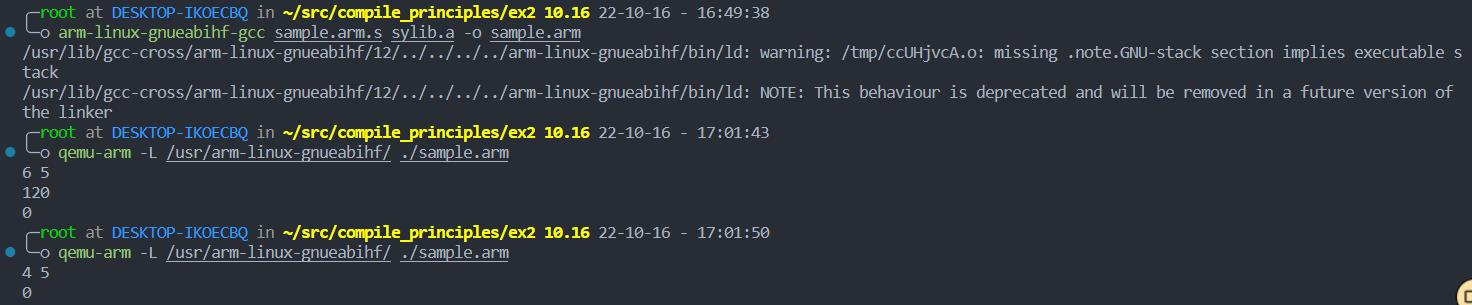
\includegraphics[width=1\textwidth]{figure/1.jpg}
  \caption{汇编代码1测试}
  \label{fig:1}
\end{figure}

根据程序设定,a <= b 和 a > b 得到的结果均正确。

\subsection{丁屹的工作}

编写的SysY示例程序如下,包含在开头列举的所有语言特性,使用了计算斐波那契数列的代码加以扩展。fib函数计算n步以后的斐波那契数,
a,b指针指向的变量保存最后两个斐波那契数,中间计算步骤保存在全局静态trace数组中。程序会向标准输入读取初始两个斐波那契数,计算步长固定为10。最后会向标准输出打印最后两个斐波那契数的和差积商以及按位与或的结果和计算步骤。

\begin{minted}[linenos,frame=lines]{c}
#include <stdio.h>

int  trace[18];
int* ptrace          = trace;
float (*nonsense)[2] = trace;
float (*ns)[2][3]    = trace;
float nnss[5][4][3][2];

void fib(int n, int* a, int* b) {
  for (int i = 0; i < n; ++i) {
    int t = *b;
    *b += *a;
    trace[i] = *b;
    *a       = t;
  }
}

int main() {
  int        a = 1, b = 1;
  const int  n         = 10;
  char       s_fmt[19] = "%d%d";
  const char p_fmt[19] = "%d %d %d %d %d %d\n";
  scanf(s_fmt, &a, &b);
  if (a > 0 && 0 < b
      || (a >= 0 || 0 <= b) && a > -1 && -1 < b && (a != 0 || 1 == b)) {
    // a > 0, b > 0 or a == 0, b == 1
    fib(n, &a, &b);
    printf(p_fmt, a + b, a - b, a * b, a / b, a & b, a | b);
    int i = 0;
    while (1) {
      printf("%d ", trace[i]);
      ++i;
      if (i == 10) {
        printf("\n");
        break;
      } else continue;
      printf("unreachable!\n");
    }
  } else {
    char err[] = "invalid input\n";
    printf(err);
    return 1;
  }
}
\end{minted}

编写对应 ARM 汇编代码及注释如下:
\begin{minted}[linenos,frame=lines]{gas}
.arch armv7-a
.fpu vfpv3-d16

.text
.global trace
.bss
.type trace, %object
.size trace, 72
trace:
.space 72

.global ptrace
.section .data.rel.local,"aw"
.type ptrace, %object
.size ptrace, 4
ptrace:
.word trace

.global nonsense
.type nonsense, %object
.size nonsense, 4
nonsense:
.word trace

.global ns
.type ns, %object
.size ns, 4
ns:
.word trace

.global nnss
.bss
.type nnss, %object
.size nnss, 480
nnss:
.space 480

.text
.global fib
.type fib, %function
fib:
  str fp, [sp, #-4]!
  add fp, sp, #0
  sub sp, sp, #28
  str r0, [fp, #-16]
  @ int n
  str r1, [fp, #-20]
  @ int* a
  str r2, [fp, #-24]
  @ int* b
  mov r3, #0
  str r3, [fp, #-8]
  @ int i = 0
  b .L0
  @ for (int i = 0; i < n; ++i)
.L1:
  ldr r3, [fp, #-24]
  @ b
  ldr r3, [r3]
  @ *b
  str r3, [fp, #-12]
  @ int t = *b
  ldr r2, [fp, #-20]
  @ a
  ldr r2, [r2]
  @ *a
  add r3, r2, r3
  ldr r2, [fp, #-24]
  str r3, [r2]
  @ *b += *a
  ldr r1, [r2]
  @ *b
  ldr r2, [fp, #-12]
  @ *a = t
  ldr r3, .LTR
.LPIC0:
  add r3, pc, r3
  ldr r2, [fp, #-8]
  @ i
  str r1, [r3, r2, lsl #2]
  @ trace[i] = *b
  ldr r3, [fp, #-20]
  @ a
  ldr r2, [fp, #-12]
  @ t
  str r2, [r3]
  @ *a = t
  ldr r3, [fp, #-8]
  add r3, r3, #1
  str r3, [fp, #-8]
  @ ++i
.L0:
  ldr r2, [fp, #-8]
  @ i
  ldr r3, [fp, #-16]
  @ n
  cmp r2, r3
  blt .L1
  @ for (...; i < n; ...)
  add sp, fp, #0
  ldr fp, [sp], #4
  bx lr
  @ return

.LTR:
.word trace-(.LPIC0+8)
.size fib, .-fib
.align 2

.global __aeabi_idiv
.section .rodata
.align 2

.LUNMSTR0:
.ascii "%d \000"
.align 2

.LSFMT:
.ascii "%d%d\000"
.space 14
.align 2

.LPFMT:
.ascii "%d %d %d %d %d %d\012\000"
.align 2

.LINVSTR:
.ascii "invalid input\012\000"
.text
.align 2

.global main
.type main, %function
main:
  push {r4, r5, r6, fp, lr}
  add fp, sp, #16
  sub sp, sp, #92
  mov r3, #1
  str r3, [fp, #-32]
  @ a = 1
  str r3, [fp, #-36]
  @ b = 1
  mov r3, #10
  str r3, [fp, #-28]
  @ n = 10
  ldr r2, .LPICT
.LPIC1:
  add r2, pc, r2
  @ char s_fmt[19] = "%d%d"
  sub r3, fp, #56
  ldm r2, {r0, r1}
  str r0, [r3]
  add r3, r3, #4
  strb r1, [r3]
  sub r3, fp, #51
  mov r2, #0
  str r2, [r3] 
  str r2, [r3, #4] 
  str r2, [r3, #8] 
  strh r2, [r3, #12] 
  ldr r3, .LPICT+4
  @ const char p_fmt[19] = "%d %d %d %d %d %d\n"
.LPIC2:
  add r3, pc, r3
  sub ip, fp, #76
  mov lr, r3
  ldmia lr!, {r0, r1, r2, r3}
  stmia ip!, {r0, r1, r2, r3}
  ldr r3, [lr]
  strh r3, [ip] 
  add ip, ip, #2
  lsr r3, r3, #16
  strb r3, [ip]
  sub r2, fp, #36
  sub r1, fp, #32
  sub r3, fp, #56
  mov r0, r3
  bl scanf(PLT)
  @ scanf(s_fmt, &a, &b)
  ldr r3, [fp, #-32]
  cmp r3, #0
  ble .L2
  @ a > 0
  ldr r3, [fp, #-36]
  cmp r3, #0
  bgt .L3
  @ 0 < b
.L2:
  ldr r3, [fp, #-32]
  cmp r3, #0
  bge .L4
  @ a >= 0
  ldr r3, [fp, #-36]
  cmp r3, #0
  blt .LINV
  @ 0 <= b
.L4:
  ldr r3, [fp, #-32]
  cmp r3, #-1
  ble .LINV
  @ a > -1
  ldr r3, [fp, #-36]
  cmp r3, #-1
  ble .LINV
  @ -1 < b
  ldr r3, [fp, #-32]
  cmp r3, #0
  bne .L3
  @ a != 0
  ldr r3, [fp, #-36]
  cmp r3, #1
  bne .LINV
  @ 1 == b
.L3:
  @ exec fib
  sub r2, fp, #36
  @ &b
  sub r3, fp, #32
  mov r1, r3
  @ &a
  ldr r0, [fp, #-28]
  @ n
  bl fib(PLT)
  @ fib
  ldr r2, [fp, #-32]
  @ a
  ldr r3, [fp, #-36]
  @ b
  add r4, r2, r3
  @ a + b
  sub r5, r2, r3
  @ a - b
  mul r6, r2, r3
  @ a * b
  mov r1, r3
  @ r1 = b
  mov r0, r2
  @ r0 = a
  bl __aeabi_idiv(PLT)
  @ r0 /= r1 -> a / b
  mov ip, r0
  ldr r1, [fp, #-32]
  @ a
  ldr r2, [fp, #-36]
  @ b
  and r3, r1, r2
  @ a & b
  orr r2, r1, r2
  @ a | b
  sub r0, fp, #76
  @ push p_fmt
  str r2, [sp, #8]
  @ push a | b
  str r3, [sp, #4]
  @ push a & b
  str ip, [sp]
  @ push a / b
  mov r3, r6
  @ push a * b
  mov r2, r5
  @ push a - b
  mov r1, r4
  @ push a + b
  bl printf(PLT)
  mov r3, #0
  str r3, [fp, #-24]
.L5:
  ldr r3, .LPICT+8
  @ "%d "
.LPIC3:
  add r3, pc, r3
  ldr r2, [fp, #-24]
  ldr r3, [r3, r2, lsl #2]
  mov r1, r3
  @ push "%d "
  ldr r0, .LPICT+12
.LPIC4:
  add r0, pc, r0
  @ push trace[i]
  bl printf(PLT)
  ldr r3, [fp, #-24]
  add r3, r3, #1
  str r3, [fp, #-24]
  @ ++i
  cmp r3, #10
  bne .L5
  @ i != 10
  mov r0, #10
  bl putchar(PLT)
  @ printf("\n") -> putchar(10)
  mov r0, #0
  b .L6
  @ printf("unreachable!\n") can be deleted
.LINV:
  ldr r3, .LPICT+16
  @ "invalid input\n"
.LPIC5:
  add r3, pc, r3
  sub ip, fp, #92
  ldm r3, {r0, r1, r2, r3}
  stmia ip!, {r0, r1, r2}
  strh r3, [ip] 
  add ip, ip, #2
  lsr r3, r3, #16
  strb r3, [ip]
  sub r3, fp, #92
  mov r0, r3
  bl printf(PLT)
  mov r0, #1
.L6:
  sub sp, fp, #16
  pop {r4, r5, r6, fp, pc}
.LPICT:
  .word .LSFMT-(.LPIC1+8)
  .word .LPFMT-(.LPIC2+8)
  .word trace-(.LPIC3+8)
  .word .LUNMSTR0-(.LPIC4+8)
  .word .LINVSTR-(.LPIC5+8)
  .size main, .-main
\end{minted}

测试代码正确性,使用 Makefile 的目标 \verb|arm-build-run| 自动构建,使用 \verb|qemu-arm| 环境模拟运行,测试如图\ref{fig:2}所示

\begin{figure}[H]
  \centering
  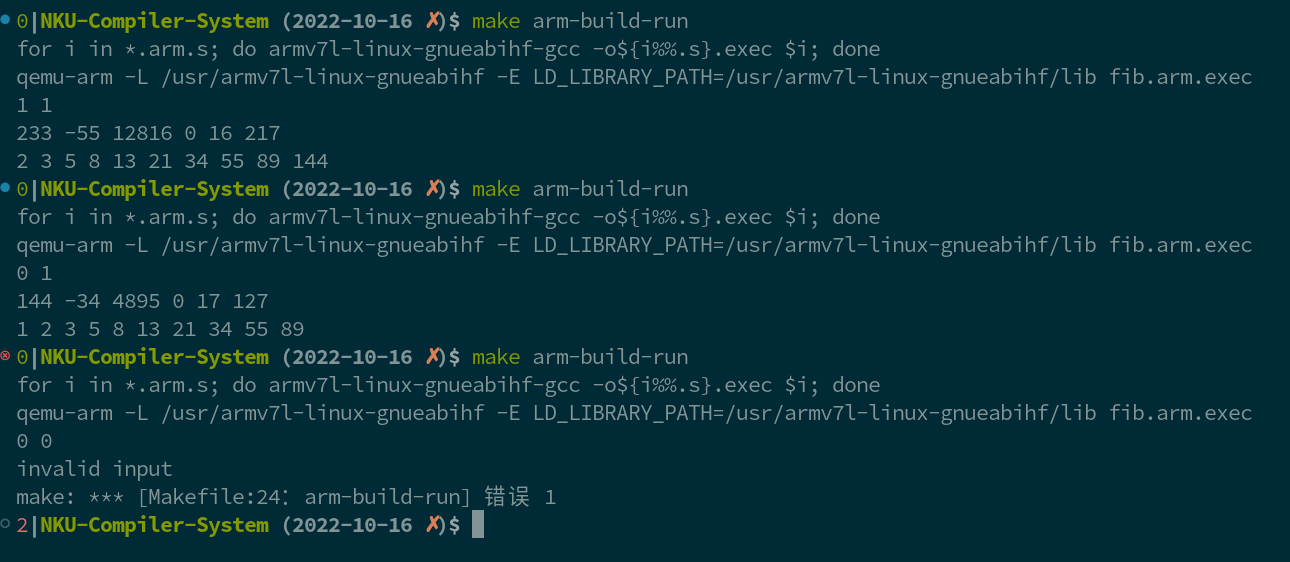
\includegraphics[width=1\textwidth]{figure/2.png}
  \caption{汇编代码2测试}
  \label{fig:2}
\end{figure}

\end{document}
